\documentclass[a4paper,titlepage]{article}
\usepackage[utf8]{inputenc}
\usepackage{fullpage}
\usepackage{indentfirst}
\usepackage[per-mode=symbol]{siunitx}
\usepackage{listings}
\usepackage{graphicx}
\usepackage{color}
\usepackage{amsmath}
\usepackage{array}
\usepackage[hidelinks]{hyperref}
\usepackage[format=plain,font=it]{caption}
\usepackage{subcaption}
\usepackage{standalone}
\usepackage[nottoc]{tocbibind}
\usepackage[nameinlink]{cleveref}
\usepackage{todonotes}
\usepackage{float}
\usepackage{algorithm}          %  float wrapper for algorithms.
\usepackage{algpseudocode}      % layout for algorithmicx
\usepackage[font=footnotesize]{caption}

% Custom commands
\newcommand\numberthis{\addtocounter{equation}{1}\tag{\theequation}}
\newcolumntype{P}[1]{>{\centering\arraybackslash}p{#1}}

\title{\textbf{COMP424: Artificial Intelligence\\ Final Project Report}}
\author{
    Weishi Wang\\
    \text{260540022}\\
    \text{wei.s.wang@mail.mcgill.ca}\\
            \text{}\\
}
\date{April 11th, 2019}

\begin{document}
\sloppy

\maketitle
\clearpage

\twocolumn

%%%%%%%%%%%%%%%%%%%%%%%%%%%%%%%%%%%%%%%%%%%%%%%%%%%%%%%%%%%%%%%%%%%%%%%%%%%%%%%%
\section{Introduction}
In this project, the goal is to implement an AI to play the game Pentago-Swap. The Pentago-Swap is a instance of Moku family of games. The game is played on a 6x6 board and consists of four 3x3 quadrants (Figure 1). The winning rule is to have 5 pieces line up in a row before the opponent does (Figure 2). The row can be vertical, horizontal and diagonal. As shown in Figure 3, at each turn, a player needs to place a piece and swap any two of the quadrants.\\

\begin{figure}[!htb]
  \centering
  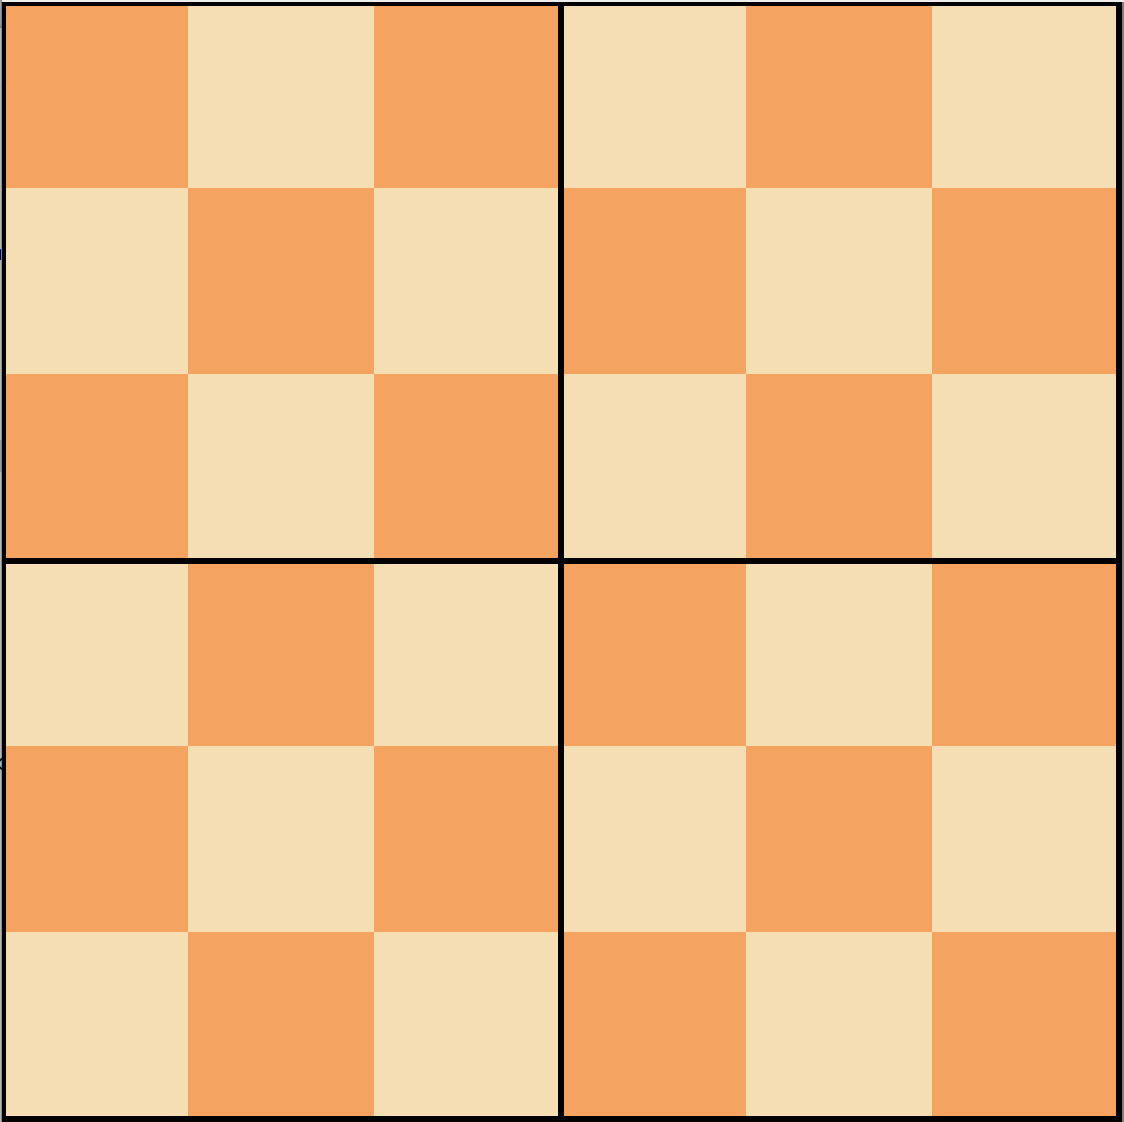
\includegraphics[width=0.4\textwidth]{image/board}
  \caption{Pentago-Swap board}
\end{figure}

\begin{figure}[!htb]
  \centering
  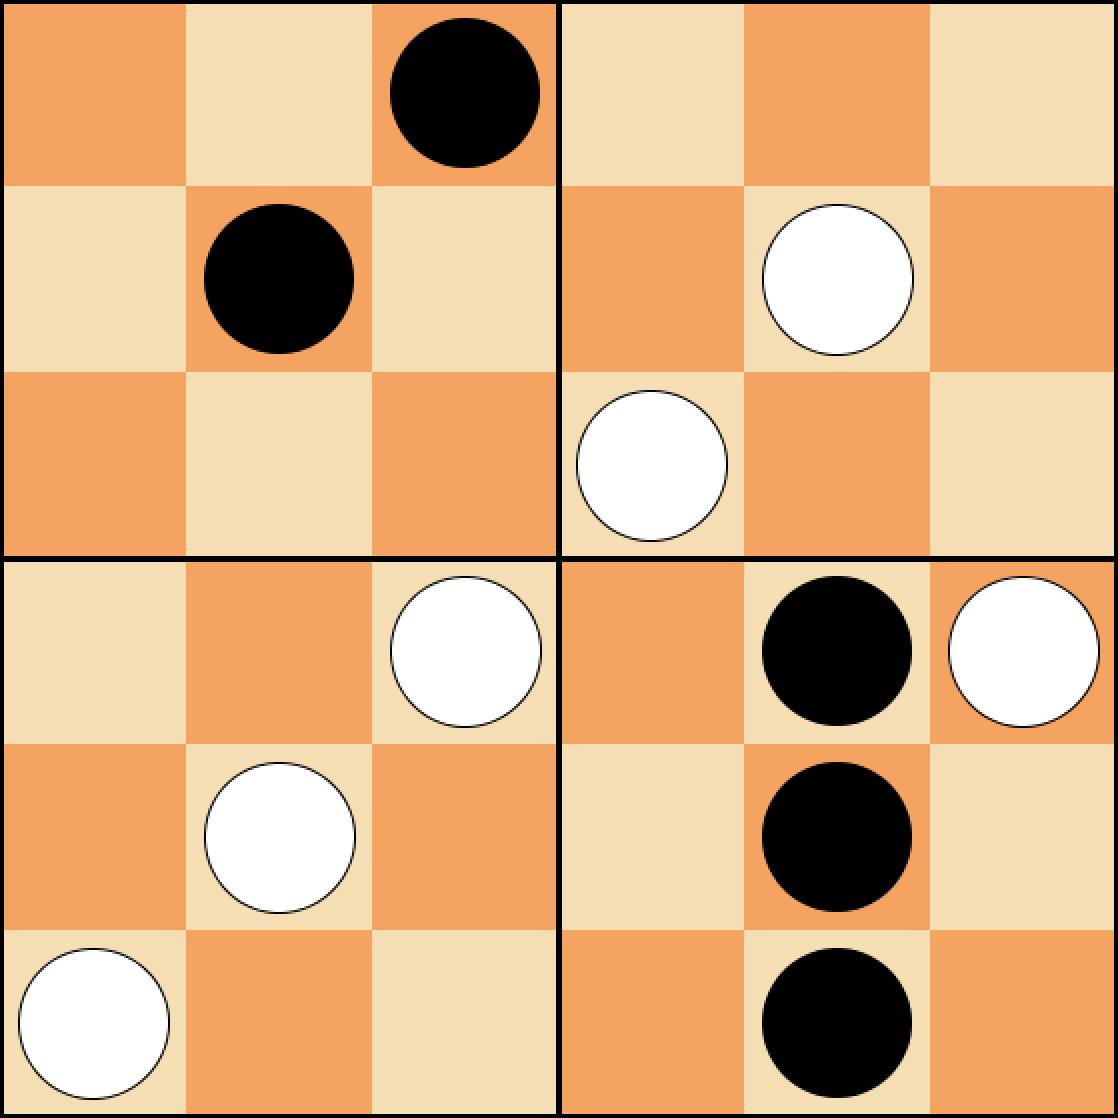
\includegraphics[width=0.4\textwidth]{image/win}
  \caption{Pentago-Swap board}
\end{figure}

\begin{figure}[!htb]
  \centering
  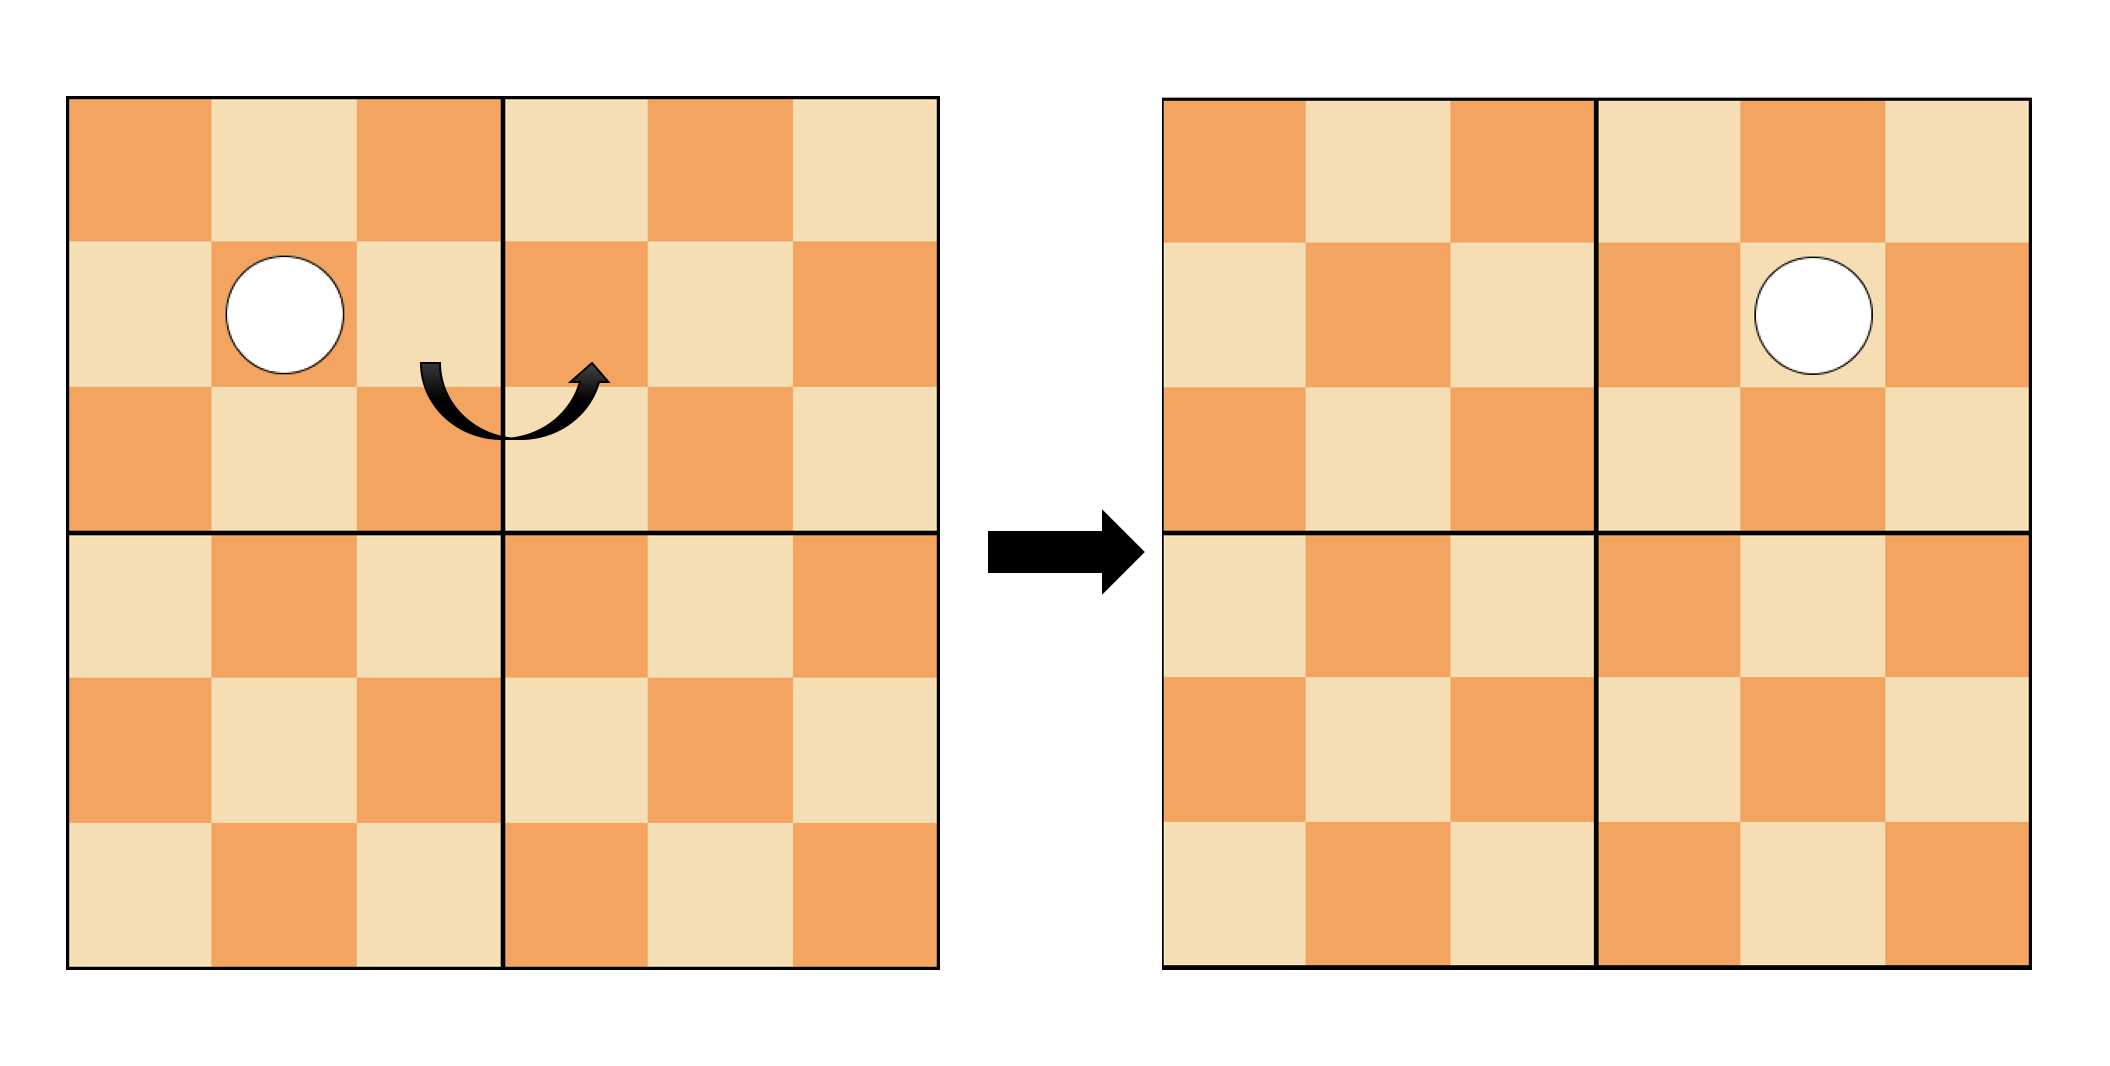
\includegraphics[width=0.55\textwidth]{image/rule}
  \caption{Pentago-Swap board}
\end{figure}


The AI created by the students are subjects to a competition at the end. There are some constraints to the competition:

\begin{enumerate}
\item Turn Timeouts : There is a initialization time at the beginning of the game, and a 2 seconds for the AI to make a move.
\item Memory Usage: The memory is not allowed to exceed 500 mb of RAM
\item Multithreading: The AI is allowed to use multi threads, however, it will run on a single processor.
\item File IO: The AI can only read files but not write files.
\end{enumerate}

Under these constraints and game rules, an AI is to be designed to win the game and compete against other AIs.

%%%%%%%%%%%%%%%%%%%%%%%%%%%%%%%%%%%%%%%%%%%%%%%%%%%%%%%%%%%%%%%%%%%%%%%%%%%%%%%%
\section{Program Explanation}

The program mainly consists of three important methods: ``$CheckWin$", ``$CheckLose$" and ``$Minimax$". The logistics of the program is to start Minimax algorithm when there is enough time to compute until the game ends. The states are given weights depending on the outcome of the game, which a win is given 1 score, a draw is 0 score and a loss is -1 score. The "CheckWin" method can detect the winning opportunity of this turn, and if there is one, it will make this move. The ``$CheckLose$" method is to detect if the opponent's next move has the possibility of winning, and block that move in the current turn. Thus, the general idea is to call "CheckWin" and "CheckLose" to play the first 8 turn, and engage "Minimax" after 8 turn. The turn number to start ``$Minimax$" is obtained by testing the program many times. When minimax starts before 8 turn, the run time will exceed 2 seconds. This chooseMove function is in the "StudentPlayer" file and the three methods are written in "MyTools" file.

\section{Motivation}
The Pentago-Swap is similar to tic-tac-toe in term of rules and strategies. For games like tic-tac-toe, it has been proven that the Minimax and Monte Carlo algorithms work well on them. The only difference between Pentago-Swap and tic-tac-toe is that Pentago-Swap has a swap phase and much more states. 

It is impossible to use Minimax on the whole game since the tree will become too large to build and impossible to search for the correct state in 2 seconds. Therefore, there are two ways to implement the Minimax algorithm in this case. The first one is to give heuristics to different winning cases and piece location, and implement Minimax to a certain depth. The weights at each depth is defined by the heuristics but not winning or losing. 

The second method to implement Minimax is to prevent losing for the first several turns and implement Minimax when there is enough time to compute all the rest state until the leaves. This is the approach that I chose for my AI at the end. 

Monte Carlo is also a good approach but it involves a simulation phase where many trials need to be fed to the algorithm. The performance of the Monte Carlo depends on the number of simulations. This might lead to poor performance because of the small number of simulations, and if we increase the number of simulations, the memory and time may run out.

Considering the pros and cons of the two algorithm, I have decided to implement the Minimax with defensive opening. The defensive opening lasts 8 turns. This number is obtained by many tests, and the Minimax with alpha-beta pruning can only compute to the end under 2 seconds after the 8th turn, which means after 16 pieces have been placed on the board. The defensive play involves of two functions: ``$CheckWin$" and "CheckLose". These two functions prevent the opponent from winning in the first 8 turns. Moreover, because of the ``$CheckWin$" function, the AI has the chance to win before the Minimax algorithm is triggered.

In general, the motivation is to implement the Minimax algorithm due to its dominant performance on tic-tac-toe. However, after evaluating the time and memory constraints, we need to make some compromises. Thus, the final choice that I made is to use defensive play before there is enough time to compute Minimax, and then use Minimax.

\section{Description and Theoretical Basis of the Approach}
In the ``$StudentPlayer$" file, the top logistic is shown in algorithm 1. The "CheckWin" method is used at the beginning of each turn to see if there is one move that leads to a win in the future. The ``$CheckLose$" method is used to check if the opponent can win in the next move. If there is a move that the opponent can win, ``$CheckLose$" will block it. After 8 turns, the ``$Minimax$" will be triggered.
\begin{algorithm}[H]
    \begin{algorithmic}[1]
    \small
        \caption{chooseMove()} \label{algorithm: choose}
        \Require boardState
         \If{$boardState.getTurn() < 8$}
         \If{$CheckWin(boardState)!= null$}
         \State return $CheckWin(boardState)$
         \Else
         \State return $CheckLose(boardState)$
         \EndIf
        \Else
        \If{$CheckWin(boardState)!= null$}
        \State return $Minimax(boardState)$
        \Else 
        \State return $CheckWin(boardState)$
        \EndIf
        \EndIf
        \end{algorithmic}
\end{algorithm}

\subsection{\small{CheckWin method}}
The three main methods shown in algorithm 1 is written in ``$MyTools$" file. The ``$CheckWin$" method takes the current boardState as input and makes a clone of the boardState. Then, it simulate all legal moves in the cloned boardState to see if the next move can lead to a win. The program returns the winning move if such a move exists, and returns null. The algorithm is shown in Algorithm 2.

\begin{algorithm}[H]
    \begin{algorithmic}[1]
    \small
        \caption{CheckWin()} \label{algorithm: win}
        \Require boardState
        \State clone = boardState.clone()
        \For{$move$ in $allLegalMoves$}
        \State $clone.process(move)$
        \If{clone wins}
        \State return move
        \EndIf
        \EndFor
        \State return null
        \end{algorithmic}
\end{algorithm}

The ``CheckWin" method is almost enough to beat the random player, unless some unfortunate random swap. Figure 4 shows an example of ``$CheckWin$" in action.

\begin{figure}[!htb]
  \centering
  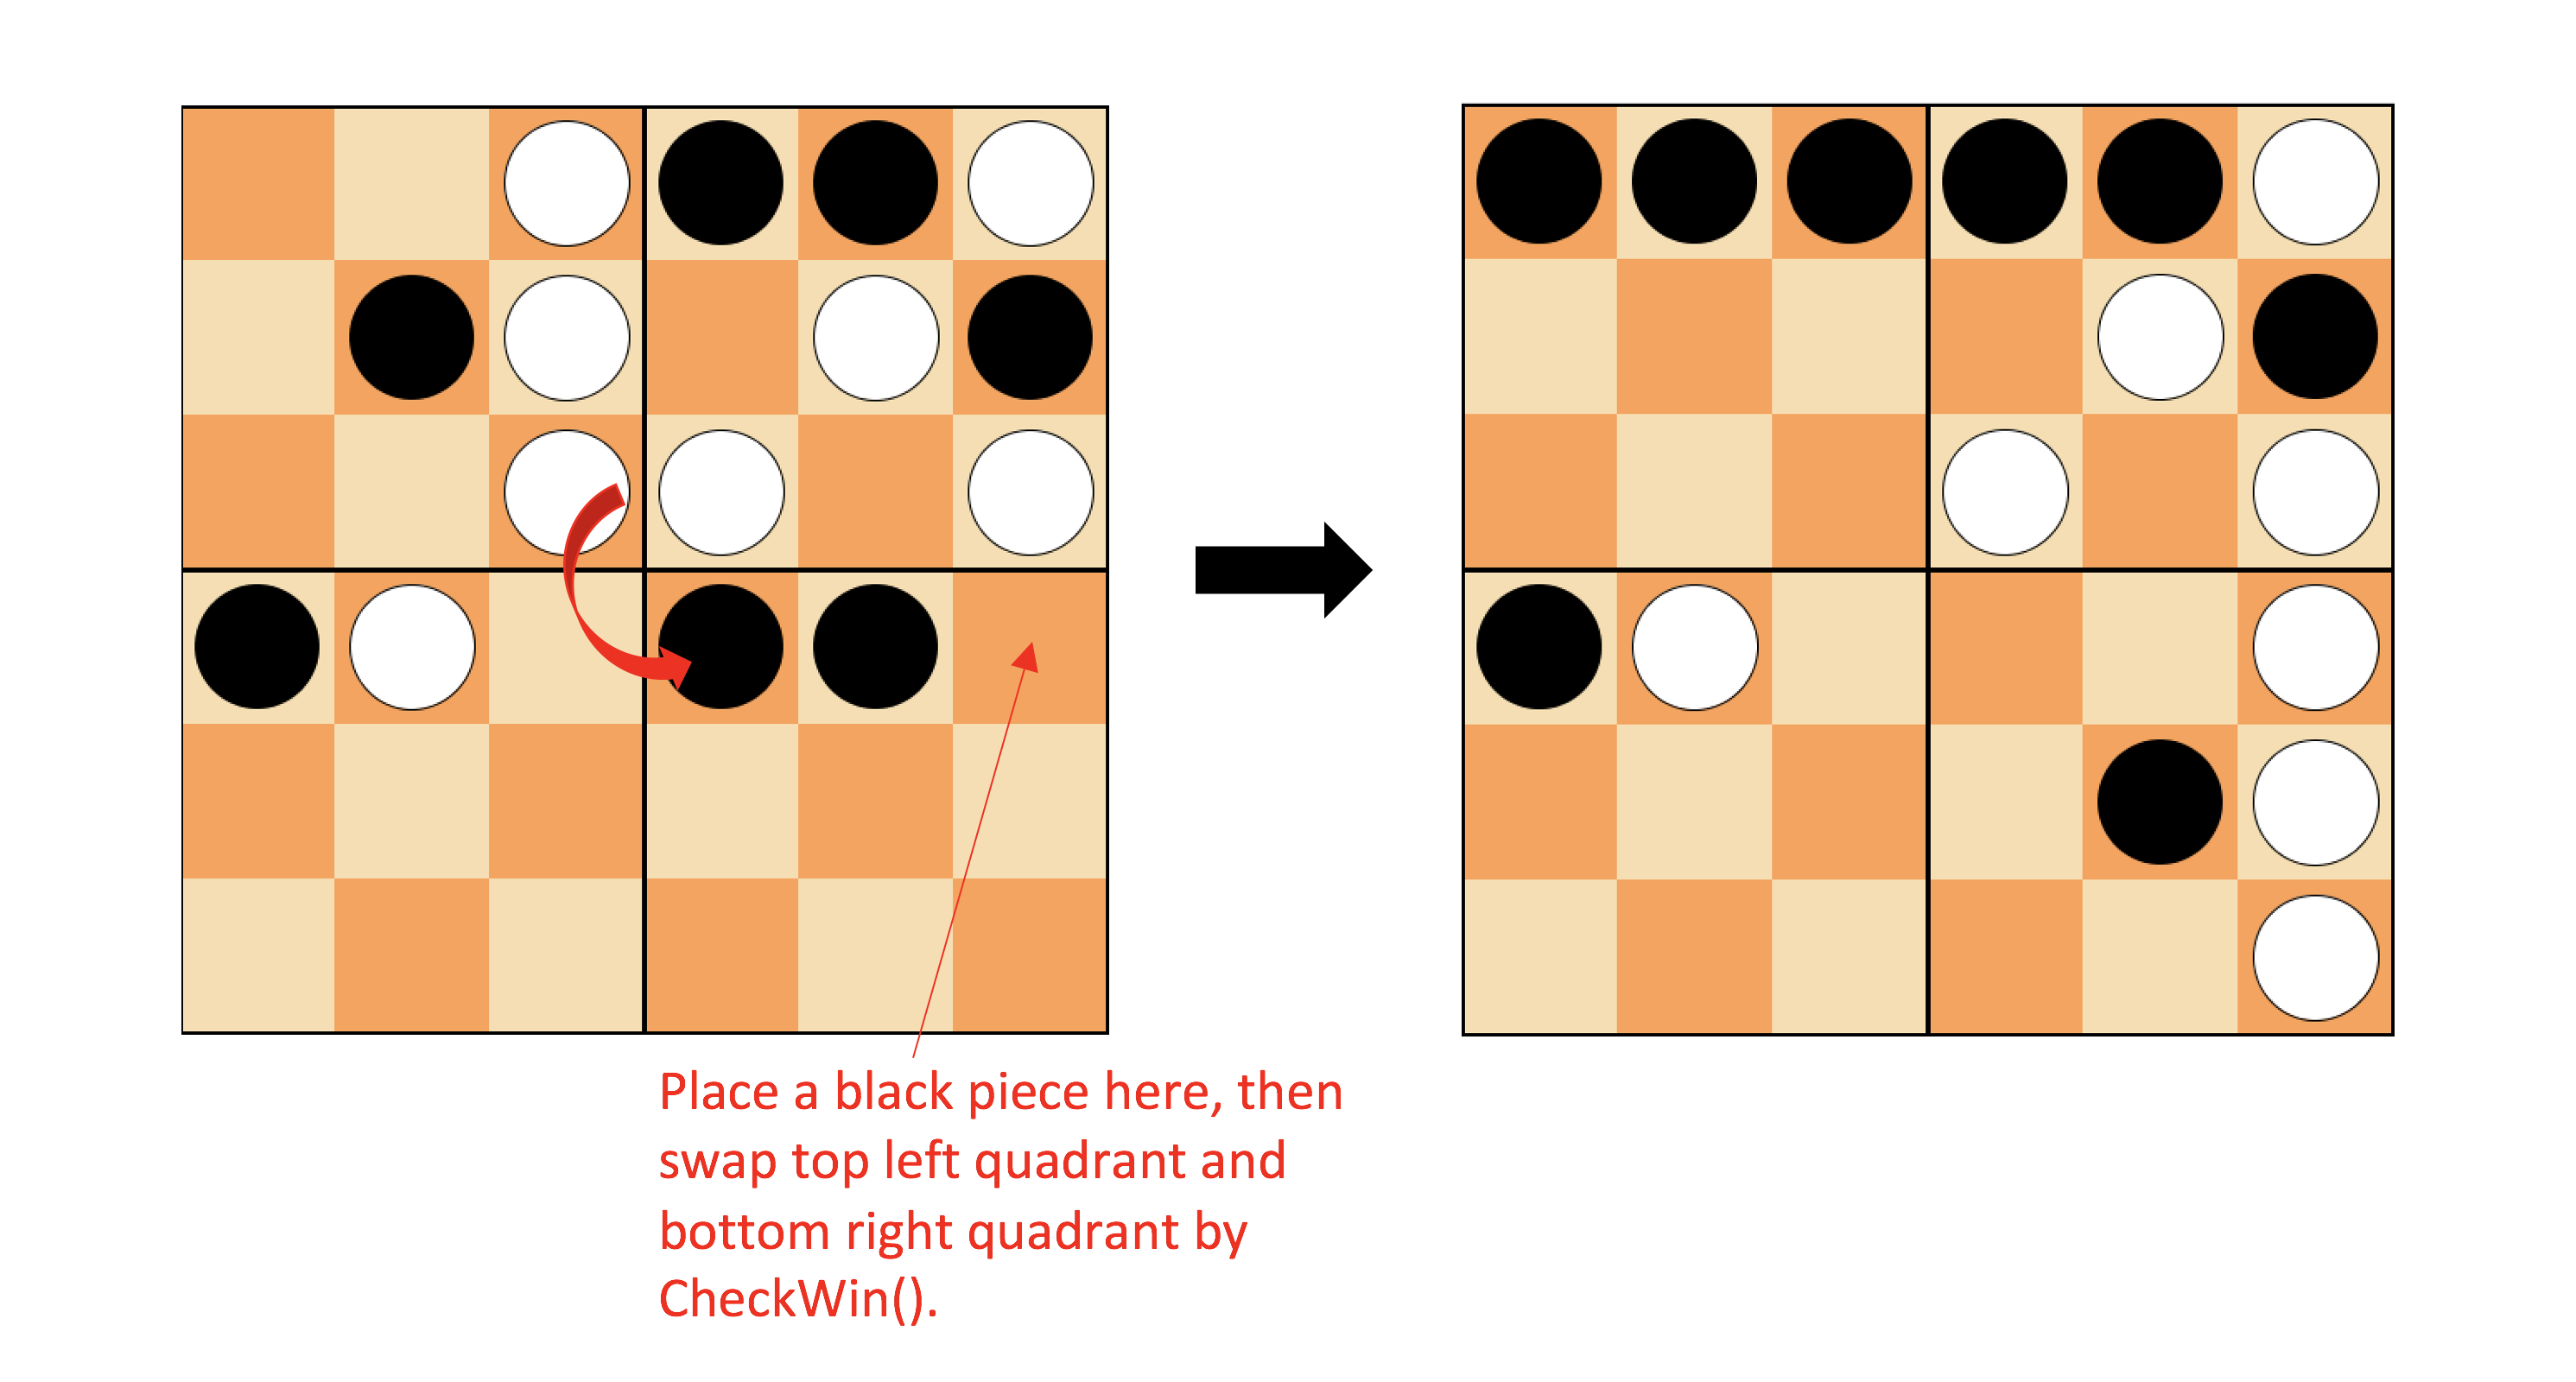
\includegraphics[width=0.5\textwidth]{image/checkwin}
  \caption{CheckWin() in action (black player is AI)}
\end{figure}


\subsection{\small{CheckLose method}}
However, only ``$CheckWin$" can not make sure of winning a random player. The ``$CheckLose$" is created to prevent opponent from winning in the next move. The ``$CheckLose$" method have a nested for loop. After cloning the current board state, we iterate over all legal moves that the AI can do. For each legal move, we iterate again over all legal moves that the opponent is allowed to make. If there exists a winning move for the opponent when we chose this move, we abandon this move. If after iterating all our moves, and there exists a winning move for the opponent in all of our legal moves, then we simply make a random move, since no matter what we do, the opponent will win if he or she is smart enough. The algorithm is shown in Algorithm 3.

\begin{algorithm}[H]
    \begin{algorithmic}[1]
    \small
        \caption{CheckLose()} \label{algorithm: lose}
        \Require boardState
        \State clone1 = boardState.clone()
        \For{$move$ in $allLegalMoves$}
        \State clone2 = clone2.clone()
         \For{$oppmove$ in $allLegalMoves$}
        \State $clone2.process(oppmove)$
        \If{clone2 wins}
        \State break
        \EndIf
        \EndFor
        \State return $move$
        \EndFor
        \State return boardState.getRandomMove()
        \end{algorithmic}
\end{algorithm}

\begin{figure}[!htb]
  \centering
  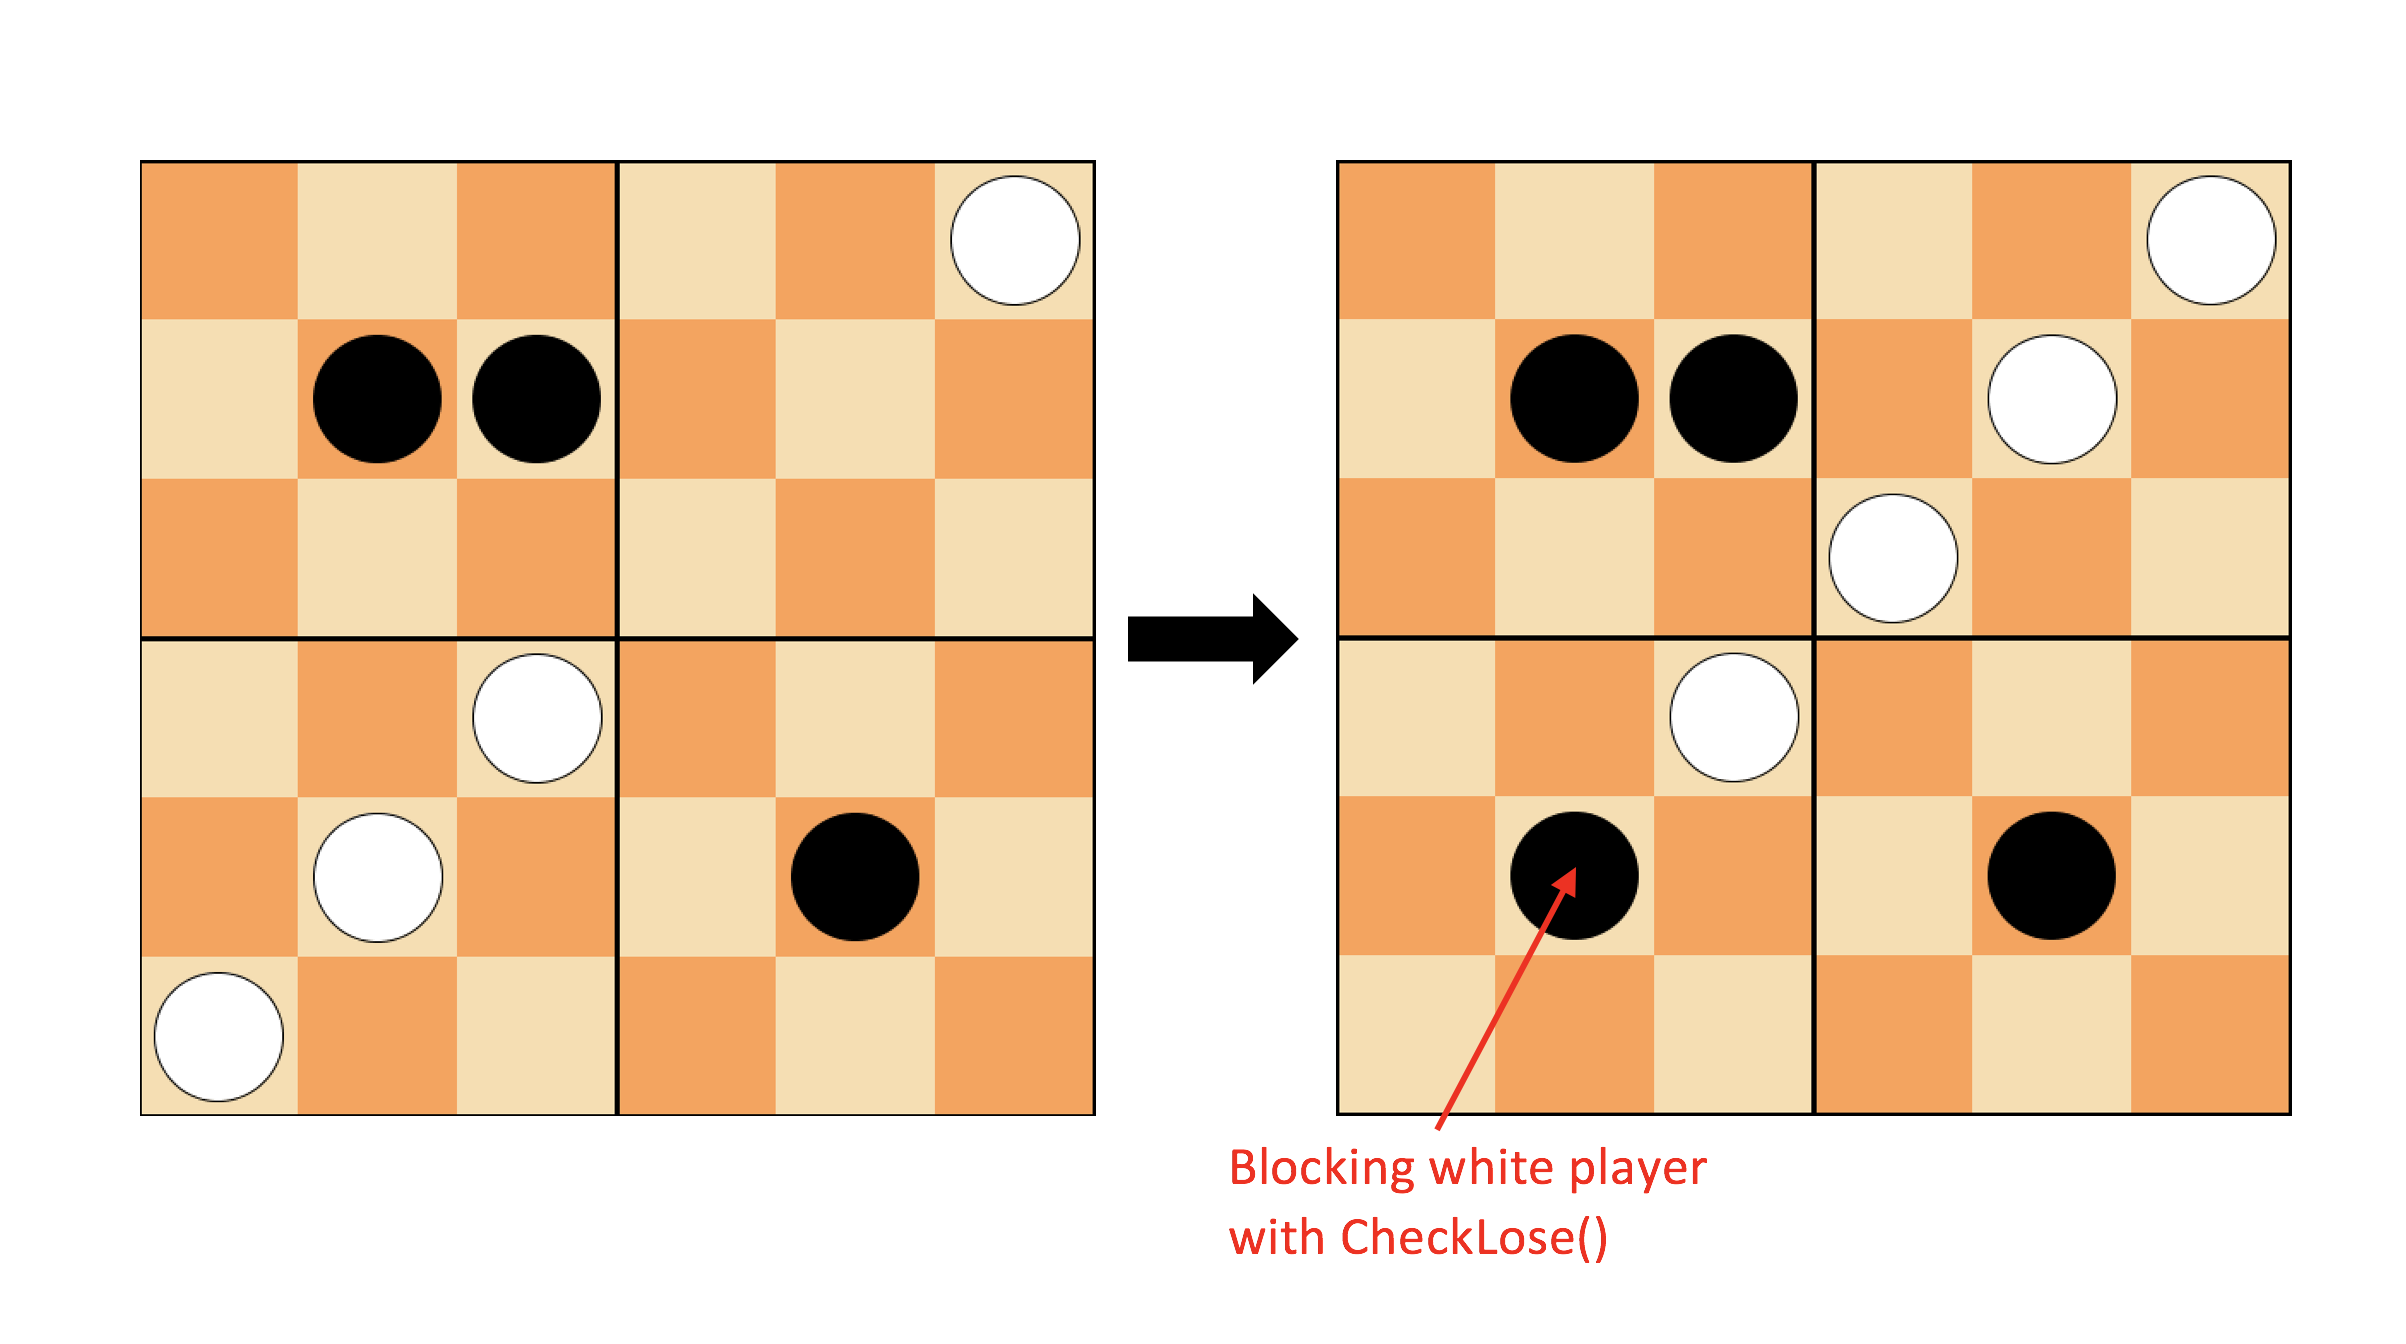
\includegraphics[width=0.5\textwidth]{image/checklose}
  \caption{CheckLose() in action (black player is AI)}
\end{figure}

After implementing both ``$CheckWin$" and ``$CheckLose$", random player has no chance of winning anymore. 100 tests have been made with ``autoplay", random player has never won once.\\

\subsection{\small{Minimax method}}
The next algorithm involved in the program is Minimax with alpha-beta pruning. Minimax is an AI algorithm that is broadly used in games [1]. The main idea of Minimax is to maximize the minimum gain, which is minimizing the possibility of loss for a worst case scenario. A crucial assumption for the Minimax algorithm is that the opponent will make the optimal move, which is not always the case.

The Minimax algorithm builds a tree of all possible states until one party wins. A positive weight is given to a winning state, a negative weight is given to a losing state and a zero is given to the draw state. The weight of different winning and losing states can be set as different weights depending on how the programmer wants to implement the Minimax algorithm. My Minimax algorithm computes the states until one party wins the whole game, and I don't take into consideration of how it wins, therefore I have given the same weight of 1 to all winning states. Similarly, I don't care how it loses, so the same negative weight of -1 is given to all losing states (Figure 6). An obvious advantage of given 1, 0 and -1 as weight and compute until the game ends is that no heuristics is required for each state. The disadvantage is that Minimax can not be started from the beginning due to the large computation. 

\begin{figure}[!htb]
  \centering
  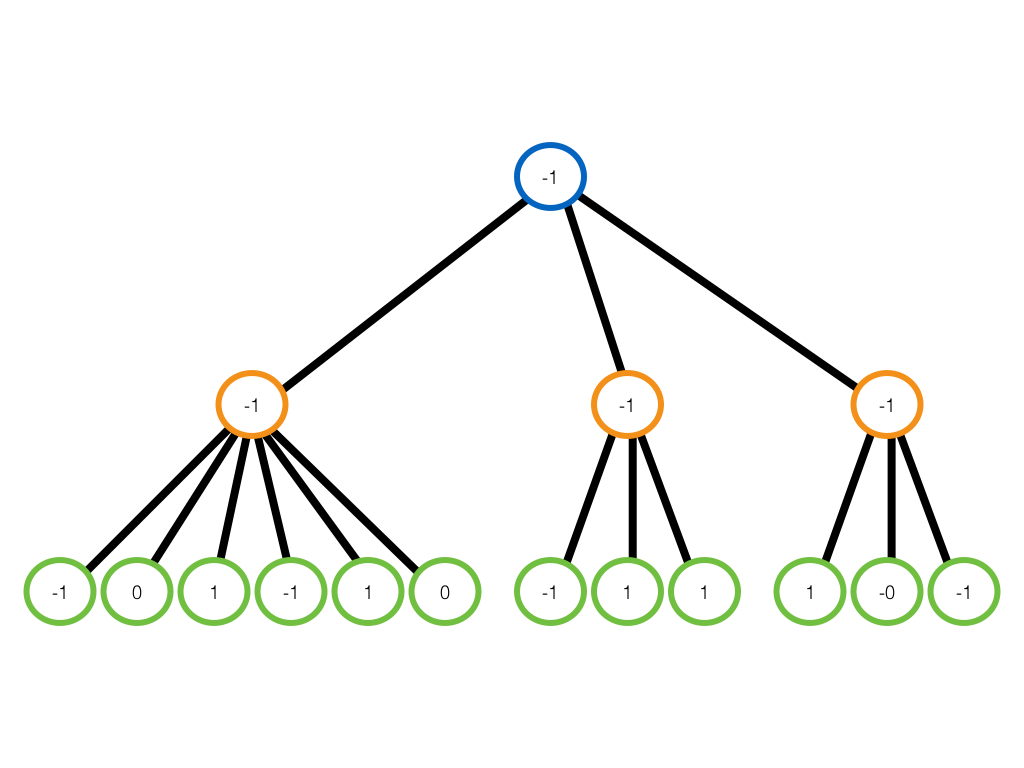
\includegraphics[width=0.4\textwidth]{image/minimax}
  \caption{Minimax that compute until the end with score of 1, 0 and -1}
\end{figure}

This might not be the case for the Minimax who computes only several layers, since it does not compute all the states until one party wins so there are actually some preferred states during the game (Figure 7). This implementation does not to compute until the game ends, and can start Minimax algorithm from the beginning of the game, but a very good and reasonable heuristics need to be given to different states.

\begin{figure}[!htb]
  \centering
  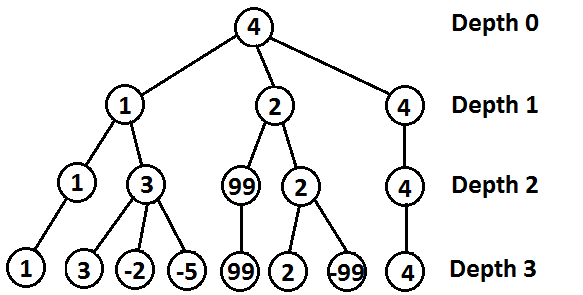
\includegraphics[width=0.4\textwidth]{image/minimaxlayers}
  \caption{Minimax that only computes to a depth of three}
\end{figure}

It is still too slow even if I start Minimax after 8 turns. There is another optimization that can be made to the state tree, alpha-beta pruning [2]. This algorithm can significantly reduce the branches of the tree by pruning the states that are worse than the current state. In other word, if a optimal state is found, all the rest states can be ignored (Figure 8).

\begin{figure}[!htb]
  \centering
  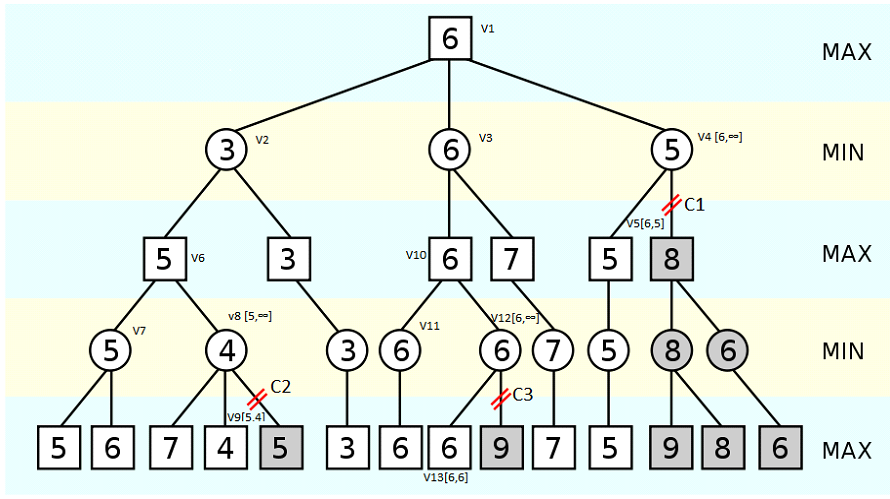
\includegraphics[width=0.5 \textwidth]{image/alpha}
  \caption{Alpha-beta pruning}
\end{figure}

The computation speed is greatly improved after implementing alpha-beta pruning, and the Minimax algorithm does not reach time out after 8 turns.

\section{Advantages and Disadvantages}

As mentioned in the section 4, the obvious advantage of my implementation is that heuristics approach can be avoided. There is no preferred winning cases or losing cases. All of them are given the same weight and considered as the same. Moreover, wrapping the ``Minimax" with a ``CheckWin" method can avoid over consider and make the winning move right away if it exists.

The disadvantage is that the opponent may very likely win within 8 turns with very smart algorithm. The defensive play before 8 turns is only checking if there exists winning case for the current state and consider losing case for the next move, however, if the opponent uses Minimax or Monte Carlo from the beginning with very good heuristics, it is likely to beat my implementation before my Minimax triggers. If the opponent is computing more than three layers, then it will beat my AI since I have only considered the current and the next steps with ``CheckWin" and ``CheckLose".

\section{Other Approaches}
Some other approaches that I have tried is Monte Carlo and Minimax with limited depth. 

\subsection{\small{Monte Carlo Approach}}
The Monte Carlo approach has the same problem as the Minimax algorithm [1]. Theoretically, it does not need heuristics since it compute until the game ends and depending on the outcome of the game, it will send back the 0 (lose) and 1 (win) to the previous nodes. After a large number of simulations, Monte Carlo can obtain moves that has higher probably of winning and will choose these moves during the game. Yet, computing the tree until the game ends is not impossible to be done in the given time frame. Therefore, same as the Minimax algorithm, heuristics need to be assigned to desired and undesired states. On top of that, Monte Carlo requires a large number of simulation to obtain relatively high performance. Thus, this approach was not chosen at the end.

\subsection{\small{Minimax With Limited Depth Approach}}
Same as the Monte Carlo approach, heuristics need to be assigned to states and many cases need to be considered, which I feel more like hard coding than artificial intelligence. After consider several state, I have moved on the my current approach.

\section{Improvements}
There are several improvements that can be made if more time is allowed for this project. After competing with some of the AIs of my classmates, I have noticed that Minimax algorithm with good heuristics have excellent performance if the state heuristic is well set. 

Therefore, one of the improvement can be wrapping up the ``CheckWin" and ``CheckLose" with Minimax that compute limited depth from the beginning, and after 8 turns, we can switch to the Minimax that computes till the end of the game. In this way, we can make sure that the opponent does not win at the first 8 turns.

Another improvement to my approach is that the Minimax could be used at the beginning with iterative deepening. This could avoid the problem of computing time as we can set the depth very small at the beginning when the branching factor is high and when the possible states decreases, we can increase the depth.

As mentioned in previous section, one reason that Minimax is not used at the beginning of the program is that a manually adjusted heuristic need to be assigned to states. This can be a painful process, but there is a way to get around it. If more time is allocated, we can use machine learning techniques to train a heuristics. We can first set the winning rule to be 3 piece in a row for the first several turns to get some reasonable heuristics for the states. Then we can increase the winning row to 4, and eventually to 5. Training can be done using deep learning by playing against itself.

In brief, there are many features that can be improved if more time is allocated for this project. The above listed points are only few ones, more specific strategies can also be implemented. 

\section{Acknowledgement}
This is a very interesting project. I would like to thank all teaching assistants and Prof. Cheung for designing this project and the competition. 

\begin{thebibliography}{99}

\bibitem{c1}Russell, Stuart J., Peter Norvig, and Ernest Davis. Artificial Intelligence: A Modern Approach. 3rd ed. Upper Saddle River, NJ: Prentice Hall, 2010. Print.

\bibitem{c2}McCarthy, John. "Human Level AI Is Harder Than It Seemed in 1955". Retrieved 2006-12-20.


\end{thebibliography}


\end{document}
